\chapter{内存管理}\label{OS03}

\section{地址、装入与保护}\label{OS03-addresses}

逻辑／虚拟地址描述进程地址空间，物理地址定位主存。OS 建立并维护映射，MMU 完成通常的运行时转换；异常进入内核处理。按字节编址时，\(v\) 位虚拟地址表示 \(2^v\) B 范围，\(p\) 位物理地址表示 \(2^p\) B 可寻址范围，实际可用量还受保留区、硬件有效位和资源约束。

\par\smallskip
{\fontsize{9.3}{12}\selectfont\setlength{\tabcolsep}{2.5pt}\setlength{\LTleft}{0pt}\setlength{\LTright}{0pt}
\begin{longtable}{@{}>{\raggedright\arraybackslash}p{\dimexpr0.41987\linewidth-2\tabcolsep\relax}>{\raggedright\arraybackslash}p{\dimexpr0.58013\linewidth-2\tabcolsep\relax}@{}}
\toprule
机制 & 工作与时机 \\

\midrule\endfirsthead\toprule
机制 & 工作与时机 \\

\midrule\endhead\bottomrule\endfoot
编译、汇编 & 生成目标模块 \\

静态链接 & 运行前连接模块并解析外部符号 \\

装入时动态链接 & 装入时连接所需模块 \\

运行时动态链接 & 运行需要时连接相应模块 \\

绝对装入 & 编译或汇编时确定绝对地址 \\

可重定位装入 & 装入时按实际起点修正有关地址 \\

动态运行时装入／重定位 & 访存时硬件按当前映射转换，可支持运行中移动 \\

\end{longtable}}
\par\smallskip

基址 \(B\)、界限为长度 \(L\) 时，先检查 \(0\le a<L\) 再形成 \(B+a\)；若界限存最大合法地址，则上界包含。上下限保护须比较物理地址，基址加界限方式可先检查逻辑地址，按寄存器定义使用。

代码、数据、堆、栈、共享库等属于虚拟映像，物理位置可离散。局部指针自身与所指堆对象分别定位，编译宏不必形成运行时对象。地址范围、驻留状态、访问权限分别检查。

\section{共享、写时复制与回收}\label{OS03-sharing}

共享页使多个进程映射到同一物理页框，虚拟页号可不同；共享只读代码可禁止写，共享可写数据仍需同步。写时复制先共享只读物理页，写入异常时，若仍须保留其他共享者的原内容，则为写者复制私有页并更新映射；若已无其他共享者，可按实现直接恢复写权限。共享页回收须检查其他使用者，映射或权限改变须使相应 TLB 项一致失效或更新。

\par\medskip\Needspace{4\baselineskip}\noindent\hypertarget{OS03-E01}{}\label{OS03-E01}\textbf{例 3-1}\par\nobreak\smallskip

进程 R 和 S 共享数据 data。若 data 在两进程中的页号分别为 p1、p2，对应页框号分别为 f1、f2，下列叙述中，正确的是（　）。

A. p1、p2 一定相等，f1、f2 一定相等

B. p1、p2 一定相等，f1、f2 不一定相等

C. p1、p2 不一定相等，f1、f2 一定相等

D. p1、p2 不一定相等，f1、f2 不一定相等

\Needspace{8\baselineskip}

\section{连续分配与动态分区}\label{OS03-partitions}

\par\smallskip
{\fontsize{9.3}{12}\selectfont\setlength{\tabcolsep}{2.5pt}\setlength{\LTleft}{0pt}\setlength{\LTright}{0pt}
\begin{longtable}{@{}>{\raggedright\arraybackslash}p{\dimexpr0.32450\linewidth-2\tabcolsep\relax}>{\raggedright\arraybackslash}p{\dimexpr0.67550\linewidth-2\tabcolsep\relax}@{}}
\toprule
方法 & 特征与碎片 \\

\midrule\endfirsthead\toprule
方法 & 特征与碎片 \\

\midrule\endhead\bottomrule\endfoot
单一连续分配 & 系统区加单个用户区，仅容纳一道用户作业 \\

固定分区 & 可等大或不等大，每区一道作业；未用区内空间为内部碎片 \\

动态分区 & 按请求划连续区；离散空洞为外部碎片 \\

\end{longtable}}
\par\smallskip

固定分区说明表保存分区号、起址、大小、状态；作业超过最大分区时，不能直接把几个离散分区拼成连续区。动态分区用空闲表或链记录起址和长度。

\par\smallskip
\begin{wideblock}
{\fontsize{9.3}{12}\selectfont\setlength{\tabcolsep}{2.5pt}\setlength{\LTleft}{0pt}\setlength{\LTright}{0pt}
\begin{longtable}{@{}>{\raggedright\arraybackslash}p{\dimexpr0.27361\linewidth-2\tabcolsep\relax}>{\raggedright\arraybackslash}p{\dimexpr0.32884\linewidth-2\tabcolsep\relax}>{\raggedright\arraybackslash}p{\dimexpr0.39755\linewidth-2\tabcolsep\relax}@{}}
\toprule
选择算法 & 查找规则及常见链序 & 主要影响 \\

\midrule\endfirsthead\toprule
选择算法 & 查找规则及常见链序 & 主要影响 \\

\midrule\endhead\bottomrule\endfoot
首次适应 & 地址递增，选首个足够大的洞 & 较可能保留高地址大洞，反复搜索低址碎片 \\

邻近／循环首次适应 & 地址循环，从上次位置继续 & 分散搜索，可能过早切分大洞 \\

最佳适应 & 选最小够用洞，常按容量递增 & 易留下难用的小碎片 \\

最坏适应 & 选最大洞，常按容量递减 & 大洞可能较快耗尽 \\

\end{longtable}}
\end{wideblock}
\par\smallskip

每次按更新后的空闲状态重新选择；空闲总量足够仍可能无足够连续洞。分配剩余区则更新起址与长度，恰好用完则删表项；回收按物理地址邻接合并：两侧均无空闲则新增，仅一侧空闲则扩展，两侧空闲则三段合一。按容量相邻的表项未必在物理地址相邻。紧凑通过搬移已分配区聚合空洞，须重定位支持并支付搬移成本。

\par\medskip\Needspace{4\baselineskip}\noindent\hypertarget{OS03-E02}{}\label{OS03-E02}\textbf{例 3-2}\par\nobreak\smallskip

某基于动态分区存储管理的计算机，主存容量为 55 MB（初始为空闲），采用最佳适配算法。分配和释放顺序为：分配 15 MB，分配 30 MB，释放 15 MB，分配 8 MB，分配 6 MB。此时最大空闲分区为（　）。

A. 7 MB　　B. 9 MB\\
C. 10 MB　　D. 15 MB

\section{覆盖、交换与虚拟存储}\label{OS03-extension}

\par\smallskip
{\fontsize{9.3}{12}\selectfont\setlength{\tabcolsep}{2.5pt}\setlength{\LTleft}{0pt}\setlength{\LTright}{0pt}
\begin{longtable}{@{}>{\raggedright\arraybackslash}p{\dimexpr0.26748\linewidth-2\tabcolsep\relax}>{\raggedright\arraybackslash}p{\dimexpr0.73252\linewidth-2\tabcolsep\relax}@{}}
\toprule
机制 & 单位与条件 \\

\midrule\endfirsthead\toprule
机制 & 单位与条件 \\

\midrule\endhead\bottomrule\endfoot
覆盖 & 常驻模块与覆盖区；同区模块不能同时需要有效内容，通常需程序员给覆盖结构 \\

交换 & 经典模型按进程映像换出、换入，挂起表示不驻留；须考虑重定位与正在进行的 I/O \\

请求调页 & 按页在实际引用时调入，利用局部性，由 OS 管理 \\

\end{longtable}}
\par\smallskip

覆盖安排：常驻 A 为8 KiB，B/C 共用最大10 KiB区，D/E/F 共用最大12 KiB区，共30 KiB；需满足给定调用和返回关系。设备正在直接访问的内存通常须固定，不能随意换出。

虚拟内存的多次性表示分批装入，对换性表示运行中可换出再换入，虚拟性表示逻辑使用空间可超过当前物理内存。容量受地址表示范围、后备能力及系统限制。仅在题给理想化模型中，可用 \(\min(\text{地址范围},\text{可用内存}+\text{可用后备})\) 估算。

\section{分页地址变换与页表空间}\label{OS03-paging}

页与页框等大，页间可映射到离散页框，页内连续；消除连续分配外部碎片，末页可有内部碎片，页表另占空间。默认字节编址，页号、页框号从0开始；容量单位按题设，本章 KiB 为 \(2^{10}\) B。

页大小 \(P\)，地址 \(a\)：

\[p=\lfloor a/P\rfloor,\qquad w=a\bmod P,\qquad PA=fP+w.\]

当 \(P=2^d\) 时，低 \(d\) 位为偏移，转换只替换页号。单级连续紧密页表基址 \(F\)、表长 \(N\) 项、每项 \(e\) B：先检查 \(0\le p<N\)，表项地址 \(F+pe\)，取页框号、驻留与权限，再访问目标；表项地址和数据地址分别计算。

\begin{figure}
\centering
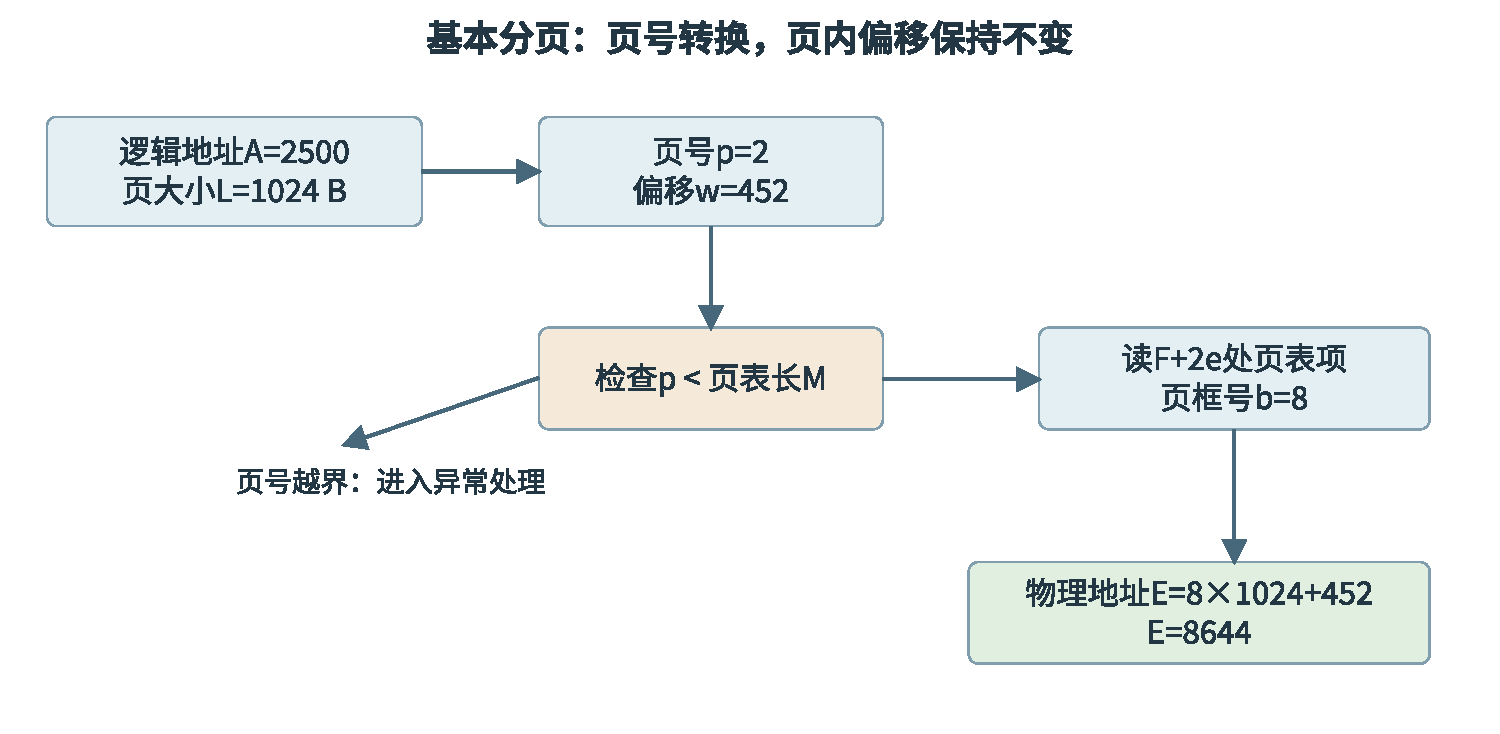
\includegraphics[width=\linewidth,height=108mm,keepaspectratio]{figures/OS_page_translation.pdf}
\caption{页号查表与页内偏移拼接}
\end{figure}

虚拟地址 \(v\) 位、物理地址 \(b\) 位、页 \(2^d\) B 时：潜在页表项 \(2^{v-d}\) 项；页框号至少 \(b-d\) 位，另加状态与权限。单级全空间页表为 \(2^{v-d}e\) B，不能用物理页框数代替虚拟页数。若每页留对齐空隙、表项不得跨页，项地址还须按实际布局计空隙。

\section{多级页表与 TLB}\label{OS03-tlb}

多级页表只为使用区间分配下级表，适合稀疏虚拟空间；全展开会增加目录开销。下级表可分散，单个最终表项宽度仍由页框和状态决定。

每表限定一页、表项 \(e\) B 时，扇出 \(q=\lfloor P/e\rfloor\)；若 \(q=2^k\)，每级最多索引 \(k\) 位页号，至少需 \(\lceil(v-d)/k\rceil\) 级。顶级可使用较少位。逐级用索引乘表项长度定位下一表，最终页框才用于数据地址。

\par\medskip\Needspace{4\baselineskip}\noindent\hypertarget{OS03-E03}{}\label{OS03-E03}\textbf{例 3-3}\par\nobreak\smallskip

某计算机采用二级页表，按字节编址，页大小为 \(2^{10}\) B，页表项大小为 2 B，逻辑地址依次由页目录号、页号、页内偏移量组成。逻辑地址空间大小为 \(2^{16}\) 页，表示整个逻辑地址空间的页目录表至少包含多少表项？

A. 64　　B. 128\\
C. 256　　D. 512

\par\medskip\Needspace{4\baselineskip}\noindent\hypertarget{OS03-E04}{}\label{OS03-E04}\textbf{例 3-4}\par\nobreak\smallskip

某计算机主存按字节编址，二级分页地址结构依次为页目录号 10 位、页号 10 位、页内偏移 12 位。虚拟地址 2050 1225H 对应的页目录号、页号分别是（　）。

A. 081H、101H　　B. 081H、401H

C. 201H、101H　　D. 201H、401H

TLB 缓存转换及权限，数据 Cache 缓存数据。TLB 未命中可从内存页表取得驻留映射；合法页不驻留才进入缺页分支。页表与 TLB 的访问、修改状态须按题给策略保持一致。

无缺页、页表各级均在内存、无其他缓存、各查询串行，TLB 查询 \(t\)、主存一次 \(m\)、命中率 \(h\)、页表 \(r\) 级：

\[E[T]=h(t+m)+(1-h)[t+(r+1)m].\]

忽略 TLB 查询时间，平均主存次数为 \(1+(1-h)r\)。并行查询须重列时间线；单级、\(t=1\ \mu s,m=100\ \mu s,h=0.9\) 时，串行111 μs；TLB 与主存页表同起，按题给命中路径101、未命中路径200 μs，则平均110.9 μs。

\section{分段与段页式}\label{OS03-segmentation}

分段按代码、数据等逻辑单位，段长可变；地址为段号、段内偏移。检查段号、段长、驻留与权限，合法后 \(PA=\text{段基址}+\text{偏移}\)。偏移等于段长即越界。

\par\smallskip
\begin{wideblock}
{\fontsize{9.3}{12}\selectfont\setlength{\tabcolsep}{2.5pt}\setlength{\LTleft}{0pt}\setlength{\LTright}{0pt}
\begin{longtable}{@{}>{\raggedright\arraybackslash}p{\dimexpr0.18118\linewidth-2\tabcolsep\relax}>{\raggedright\arraybackslash}p{\dimexpr0.43447\linewidth-2\tabcolsep\relax}>{\raggedright\arraybackslash}p{\dimexpr0.38435\linewidth-2\tabcolsep\relax}@{}}
\toprule
机制 & 地址与表路径 & 物理布局、碎片 \\

\midrule\endfirsthead\toprule
机制 & 地址与表路径 & 物理布局、碎片 \\

\midrule\endhead\bottomrule\endfoot
基本分页 & 页号、页内偏移；页表→目标 & 页内连续、页间离散，内部碎片 \\

基本分段 & 段号、段内偏移；段表→目标 & 每段连续、段间离散，外部碎片 \\

段页式 & 段号、段内页号、页内偏移；段表→本段页表→目标 & 段内页可离散，各段末页可能有内部碎片 \\

\end{longtable}}
\end{wideblock}
\par\smallskip

上述单级各表驻留、无 TLB 及其他缓存、无异常时分别2、2、3次主存访问。段页式逻辑坐标仍可视为段号、段内地址二维；编码可把段内地址拆为两个字段。先查段范围权限，再查段内页范围；题给字节段长时还须检查完整段内偏移。

\section{请求分页与缺页处理}\label{OS03-demand-paging}

时间局部性来自重复使用，空间局部性来自邻近访问。请求分页页表记录存在位、访问位 A、修改位 M、后备位置及保护信息。M 表示已写，写权限表示能否写，二者独立。

合法地址查询 \ensuremath{\to} 页未驻留 \ensuremath{\to} 保存重启状态并定位后备页 \ensuremath{\to} 取得空框或选择牺牲页 \ensuremath{\to} 必要时写回脏页 \ensuremath{\to} 调入 \ensuremath{\to} 更新页表、失效旧 TLB 并建立新转换 \ensuremath{\to} 重试原指令。权限不足或非法地址按保护错误处理。

\begin{figure}
\centering
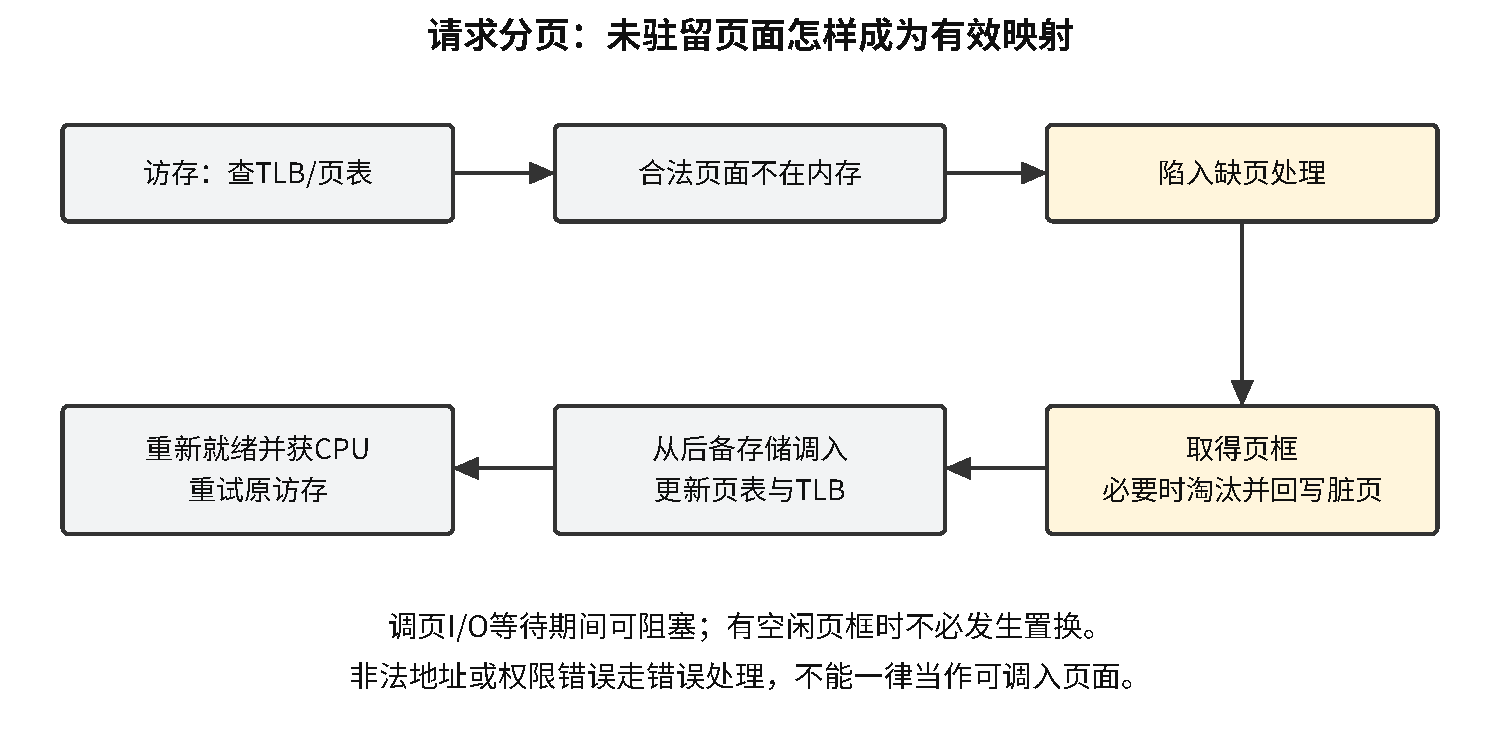
\includegraphics[width=\linewidth,height=108mm,keepaspectratio]{figures/OS_page_fault.pdf}
\caption{缺页处理与原指令重试}
\end{figure}

有空框的缺页无需置换；干净且有有效后备副本的牺牲页可直接丢弃；需保留的脏内容在复用页框前回写。一条复杂指令可引用多页、产生多次缺页，最少页框数须满足指令及寻址重启要求。锁定内核页和正在供设备直接访问的页通常不参与置换。

\section{页框分配与页面后备}\label{OS03-resident-allocation}

驻留集是当前在物理内存的页面集合。固定分配保持进程页框数，可变分配按运行调整；局部置换仅选本进程页面，全局置换可影响其他进程的页框占用。经典组合为固定分配局部置换、可变分配局部置换、可变分配全局置换。页框可平均、按大小或按优先级分配，仍须满足最少页框要求。

请求调页在引用时调入，预调页提前装入预计会使用的页；预调有无用 I/O 风险。后备位置模型：对换区充分时可先复制到对换区，运行中在内存和对换区交换；对换区不足时只读文件页从文件读、淘汰丢弃，修改内容写入对换区；教材 UNIX 模型首次从文件调入、已换出者从对换区调回。匿名页、私有映射、共享文件映射具体后备关系按题设。

\section{页面置换算法}\label{OS03-replacement}

\par\smallskip
\begin{wideblock}
{\fontsize{9.3}{12}\selectfont\setlength{\tabcolsep}{2.5pt}\setlength{\LTleft}{0pt}\setlength{\LTright}{0pt}
\begin{longtable}{@{}>{\raggedright\arraybackslash}p{\dimexpr0.20703\linewidth-2\tabcolsep\relax}>{\raggedright\arraybackslash}p{\dimexpr0.39416\linewidth-2\tabcolsep\relax}>{\raggedright\arraybackslash}p{\dimexpr0.39881\linewidth-2\tabcolsep\relax}@{}}
\toprule
算法 & 淘汰依据 & 状态更新与边界 \\

\midrule\endfirsthead\toprule
算法 & 淘汰依据 & 状态更新与边界 \\

\midrule\endhead\bottomrule\endfoot
OPT & 未来最久不用或以后不用 & 理论比较下界，需未来引用串 \\

FIFO & 最早装入 & 命中不改变装入队列；可有 Belady 异常 \\

LRU & 过去最久未使用 & 每次命中都更新最近次序，实现需额外记录 \\

Clock & 循环扫描 A=0 者；A=1 清零并跳过 & 命中置 A=1；装入、指针规则采用题设 \\

改进 Clock & 同时考虑 A、M，优先近期未访问且干净者 & 扫描只清 A，脏内容回写后才可清 M \\

\end{longtable}}
\end{wideblock}
\par\smallskip

LRU、OPT 在相同引用串和一致初态下具有栈性质，增框不会增加缺页；LRU 对任意串优于 FIFO 的结论不成立。缺页总数分为使用空框与淘汰旧页两类，置换次数须扣除空框初装。

\par\medskip\Needspace{4\baselineskip}\noindent\hypertarget{OS03-E05}{}\label{OS03-E05}\textbf{例 3-5}\par\nobreak\smallskip

某系统采用 LRU 页置换和局部置换。为进程预分配 4 个页框，访问页号依次为 0、1、2、7、0、5、3、5、0、2、7、6。产生页面置换的总次数为（　）。

A. 3　　B. 4\\
C. 5　　D. 6

教材改进 Clock 四轮：{\SNsymbolfont ①}自起点找首个 \((0,0)\)，不改 A；{\SNsymbolfont ②}找首个 \((0,1)\)，经过但未选中的页 A 清零；{\SNsymbolfont ③}若仍失败，重新从起点找 \((0,0)\)，不改 A；{\SNsymbolfont ④}再找 \((0,1)\)。每轮最多一圈；第2轮改变了后续候选分类，须动态更新。起点与指针推进规则决定同类中选择哪个页。

\par\medskip\Needspace{4\baselineskip}\noindent\hypertarget{OS03-E06}{}\label{OS03-E06}\textbf{例 3-6}\par\nobreak\smallskip

某请求分页系统页大小为 4 KB，按字节编址。为进程 P 分配 2 个固定页框，采用改进型 Clock，页表部分内容如下。

\par\smallskip
{\fontsize{9.3}{12}\selectfont\setlength{\tabcolsep}{2.5pt}\setlength{\LTleft}{0pt}\setlength{\LTright}{0pt}
\begin{longtable}{@{}>{\raggedright\arraybackslash}p{\dimexpr0.25000\linewidth-2\tabcolsep\relax}>{\raggedright\arraybackslash}p{\dimexpr0.25000\linewidth-2\tabcolsep\relax}>{\raggedright\arraybackslash}p{\dimexpr0.25000\linewidth-2\tabcolsep\relax}>{\raggedright\arraybackslash}p{\dimexpr0.25000\linewidth-2\tabcolsep\relax}@{}}
\toprule
页号 & 页框号 & 存在位 & 访问位 \\

\midrule\endfirsthead\toprule
页号 & 页框号 & 存在位 & 访问位 \\

\midrule\endhead\bottomrule\endfoot
2 & 20H & 0 & 0 \\

3 & 60H & 1 & 1 \\

4 & 80H & 1 & 1 \\

\end{longtable}}
\par\smallskip

\par\smallskip
{\fontsize{9.3}{12}\selectfont\setlength{\tabcolsep}{2.5pt}\setlength{\LTleft}{0pt}\setlength{\LTright}{0pt}
\begin{longtable}{@{}>{\raggedright\arraybackslash}p{\dimexpr0.50000\linewidth-2\tabcolsep\relax}>{\raggedright\arraybackslash}p{\dimexpr0.50000\linewidth-2\tabcolsep\relax}@{}}
\toprule
页号 & 修改位 \\

\midrule\endfirsthead\toprule
页号 & 修改位 \\

\midrule\endhead\bottomrule\endfoot
2 & 0 \\

3 & 0 \\

4 & 1 \\

\end{longtable}}
\par\smallskip

P 访问虚拟地址 02A01H，经地址变换得到的物理地址是（　）。

A. 00A01H　　B. 20A01H\\
C. 60A01H　　D. 80A01H

\section{工作集、抖动与数组局部性}\label{OS03-working-set}

工作集是最近窗口内访问过的不同页集合；按最近 \(\Delta\) 次引用定义时，先取引用再去重，集合大小可小于窗口。驻留集反映物理状态，工作集反映近期需求；工作集未必总为驻留集子集。

\par\medskip\Needspace{4\baselineskip}\noindent\hypertarget{OS03-E07}{}\label{OS03-E07}\textbf{例 3-7}\par\nobreak\smallskip

某进程访问页面的序列如下，t 位于所示竖线处，尚未访问竖线右侧的 0。

\[\ldots,1,3,4,5,6,0,3,2,3,2\;\big|_{t}\;0,4,0,3,2,9,2,1,\ldots\]

工作集窗口大小为 6，则 t 时刻工作集为（　）。

A. \{6,0,3,2\}　　B. \{2,3,0,4\}\\
C. \{0,4,3,2,9\}　　D. \{4,5,6,0,3,2\}

总工作集需求超过可用页框可引发抖动，大量时间用于换页、计算进展少。可减少活动进程、增加相应页框或用工作集／缺页率调节；扩充交换区容量无法直接补足驻留页框。

行优先数组元素 \texttt{a[\allowbreak{}i]\allowbreak{}[\allowbreak{}j]\allowbreak{}} 字节偏移为 \((i\cdot\text{列数}+j)\cdot\text{元素字节数}\)。先加起始地址、再分解页号，形成引用串；缺页数还依初态、对齐、页框和置换。4 B 整数、页对齐 \texttt{a[\allowbreak{}128]\allowbreak{}[\allowbreak{}128]\allowbreak{}}、页512 B、仅1个数据页框且初始未装入时：行遍历每行一缺页共128次，列遍历每次跨行共16384次。

\section{有效访问时间与综合地址计算}\label{OS03-effective-time}

无缺页平均耗时 \(T_0\)、缺页率 \(p\)、完整缺页分支耗时 \(T_f\)：

\[E[T]=(1-p)T_0+pT_f.\]

若服务时间 \(D\) 定义为正常访存外的附加量，可用 \(E[T]=T_0+pD\)。逐项确认失败查询、调入、脏页回写、表更新与重试是否已含；统一 ns、μs、ms。TLB 命中率与缺页率按条件路径组合。

\par\medskip\Needspace{4\baselineskip}\noindent\hypertarget{OS03-E08}{}\label{OS03-E08}\textbf{例 3-8}\par\nobreak\smallskip

请求分页管理系统中，假设某进程的页表内容如下表所示。

\par\smallskip
{\fontsize{9.3}{12}\selectfont\setlength{\tabcolsep}{2.5pt}\setlength{\LTleft}{0pt}\setlength{\LTright}{0pt}
\begin{longtable}{@{}>{\raggedright\arraybackslash}p{\dimexpr0.29289\linewidth-2\tabcolsep\relax}>{\raggedright\arraybackslash}p{\dimexpr0.29289\linewidth-2\tabcolsep\relax}>{\raggedright\arraybackslash}p{\dimexpr0.41421\linewidth-2\tabcolsep\relax}@{}}
\toprule
页号 & 页框号 & 有效位（存在位） \\

\midrule\endfirsthead\toprule
页号 & 页框号 & 有效位（存在位） \\

\midrule\endhead\bottomrule\endfoot
0 & 101H & 1 \\

1 & --- & 0 \\

2 & 254H & 1 \\

\end{longtable}}
\par\smallskip

页面大小为 4 KB，一次内存的访问时间为 100 ns，一次快表（TLB）的访问时间为 10 ns，处理一次缺页的平均时间为 \(10^8\) ns（已含更新 TLB 和页表的时间）。进程的驻留集大小固定为 2，采用最近最少使用置换算法（LRU）和局部淘汰策略。假设：{\SNsymbolfont ①}TLB 初始为空；{\SNsymbolfont ②}地址转换时先访问 TLB，若 TLB 未命中，再访问页表（忽略访问页表之后的 TLB 更新时间）；{\SNsymbolfont ③}有效位为 0 表示页面不在内存中，产生缺页中断，缺页中断处理后，返回到产生缺页中断的指令处重新执行。设有虚地址访问序列 2362H、1565H、25A5H，请问：

（1）依次访问上述三个虚地址，各需多少时间？给出计算过程。

（2）基于上述访问序列，虚地址 1565H 的物理地址是多少？请说明理由。

\par\medskip\Needspace{4\baselineskip}\noindent\hypertarget{OS03-E09}{}\label{OS03-E09}\textbf{例 3-9}\par\nobreak\smallskip

某 32 位系统采用基于二级页表的请求分页存储管理方式，按字节编址，页目录项和页表项长度均为 4 字节，虚拟地址结构如下所示。

\par\smallskip
{\fontsize{9.3}{12}\selectfont\setlength{\tabcolsep}{2.5pt}\setlength{\LTleft}{0pt}\setlength{\LTright}{0pt}
\begin{longtable}{@{}>{\raggedright\arraybackslash}p{\dimexpr0.34104\linewidth-2\tabcolsep\relax}>{\raggedright\arraybackslash}p{\dimexpr0.29855\linewidth-2\tabcolsep\relax}>{\raggedright\arraybackslash}p{\dimexpr0.36041\linewidth-2\tabcolsep\relax}@{}}
\toprule
页目录号（10 位） & 页号（10 位） & 页内偏移量（12 位） \\

\midrule\endfirsthead\toprule
页目录号（10 位） & 页号（10 位） & 页内偏移量（12 位） \\

\midrule\endhead\bottomrule\endfoot
\end{longtable}}
\par\smallskip

某 C 程序中数组 \texttt{a[\allowbreak{}1024]\allowbreak{}[\allowbreak{}1024]\allowbreak{}} 的起始虚拟地址为 1080 0000H，数组元素占 4 字节，该程序运行时，其进程的页目录起始物理地址为 0020 1000H。请回答下列问题。

（1）数组元素 \texttt{a[\allowbreak{}1]\allowbreak{}[\allowbreak{}2]\allowbreak{}} 的虚拟地址是什么？对应的页目录号和页号分别是什么？对应的页目录项的物理地址是什么？若该目录项中存放的页框号为 00301H，则 \texttt{a[\allowbreak{}1]\allowbreak{}[\allowbreak{}2]\allowbreak{}} 所在页对应的页表项的物理地址是什么？

（2）数组 a 在虚拟地址空间中所占的区域是否必须连续？在物理地址空间中所占区域是否必须连续？

（3）已知数组 a 按行优先方式存放，若对数组 a 分别按行遍历和按列遍历，则哪种遍历方式的局部性更好？

\section{内存映射文件}\label{OS03-mmap}

文件范围关联进程虚拟范围，应用用普通访存访问，系统按需驻留和写回。共享映射可指向相同文件页，修改共享数据须同步；私有映射可用写时复制。建立映射、页面驻留和脏页持久化分别发生。统计设备 I/O 时检查缓存、缺页、写回及后备位置。
